\chapter{Results}
\label{chap:results}

\begin{figure}
	\centering
	\subfloat[Snail - 1 topmost csg node]{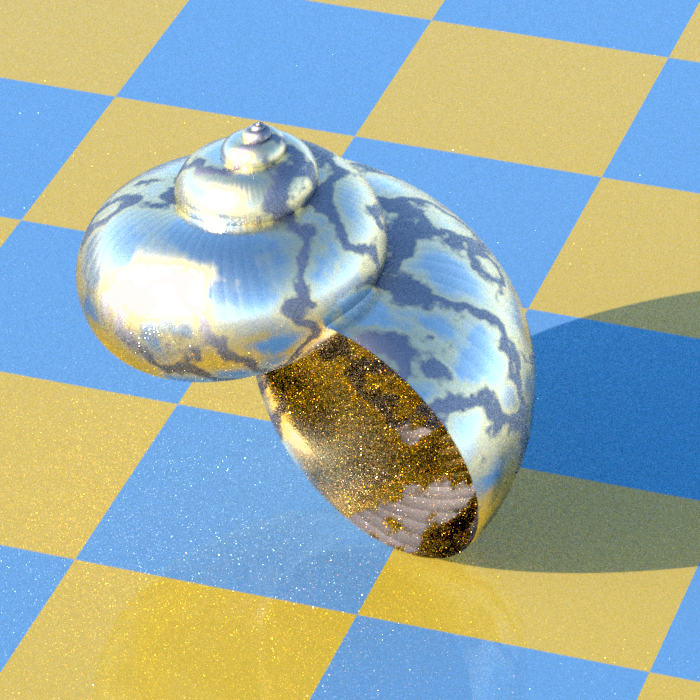
\includegraphics[width=.3\textwidth]{img/4 results/csg/snailEmbree.png}\label{fig:csg_snail}}
	\hfill
	\subfloat[Oren Nayar Sphreres - 3 topmost csg nodes]{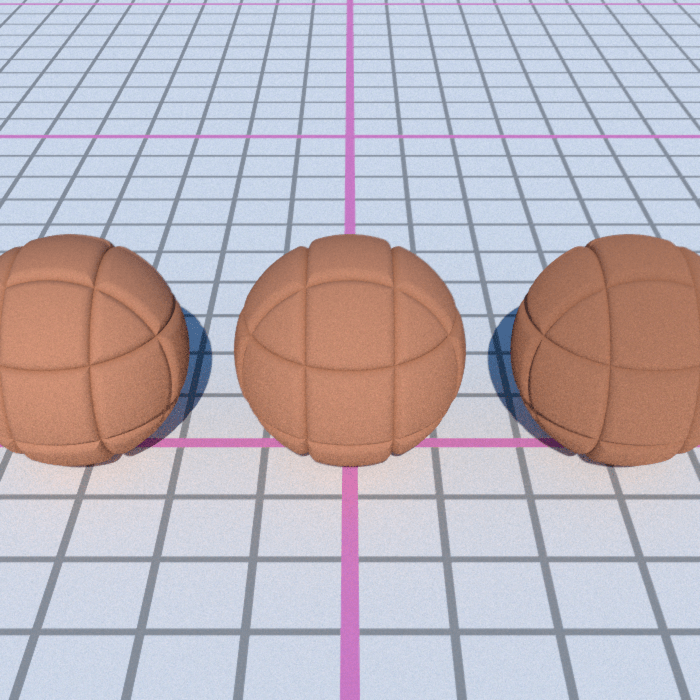
\includegraphics[width=.3\textwidth]{img/4 results/csg/orennayarEmbree.png}\label{fig:csg_orennayar}}
	\hfill
	\subfloat[Villa Rotonda - 2 topmost csg nodes.]{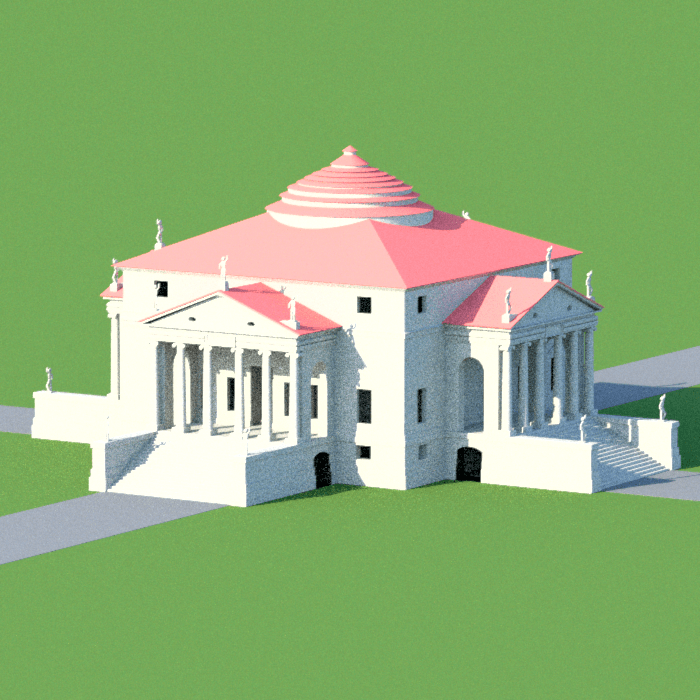
\includegraphics[width=.3\textwidth]{img/4 results/csg/rotondaEmbree.png}\label{fig:mesh_rotonda}}
	\\
	\subfloat[Torrance Sparrow Spheres - 12 topmost csg nodes.]{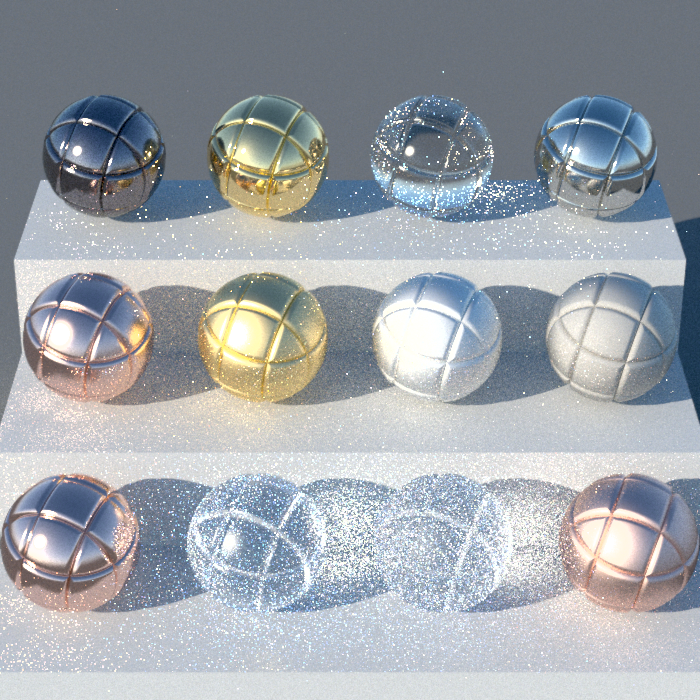
\includegraphics[width=.3\textwidth]{img/4 results/csg/torrancesparrowEmbree.png}\label{fig:csg_torrancesparrow}}
	\hfill
	\subfloat[Parked Biplane - 28 topmost csg nodes.]{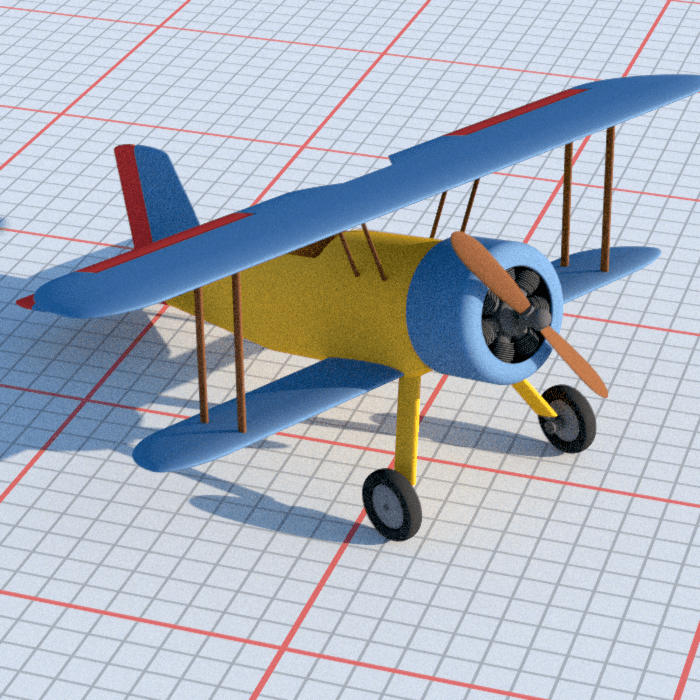
\includegraphics[width=.3\textwidth]{img/4 results/csg/planeEmbree.png}\label{fig:csg_plane}}
	\hfill
	\subfloat[Locomotive Scene - 354 topmost csg nodes]{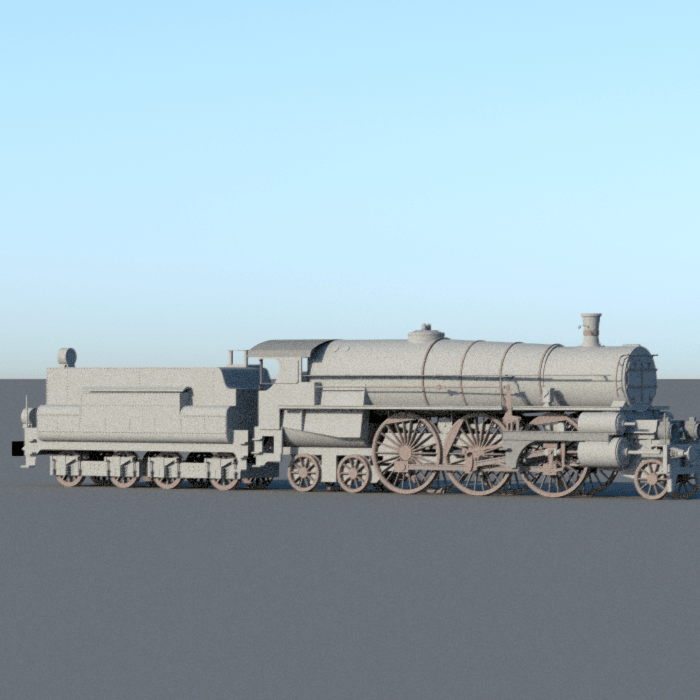
\includegraphics[width=.3\textwidth]{img/4 results/csg/locomotiveEmbree.png}\label{fig:csg_locomotive}}
	
	\caption{Scenes for csg rendering}
	\label{fig:csg_figures}
\end{figure}

\begin{table}
	\centering
	{\footnotesize\sf
		\begin{tabular}{lrrrrrr}
			\toprule
			Scene & \Verb!#!CSG & Native ART & Approach 2 & Speedup 2 & Approach 3 & Speedup 3 \\ 
			\midrule
			Figure \ref{fig:csg_snail} & 1 & 2,611.75 sec & 2,437.81 sec & 6.66 \% & 4,151.01 sec & \textcolor{red}{-58.94 \%}  \\
			Figure \ref{fig:csg_orennayar} & 3 & 791.71 sec & 522.97 sec & 33.94 \% & 528.77 sec & 33.21 \% \\
			Figure \ref{fig:mesh_rotonda} & 2 & 738.25 sec & 629.03 sec & 14.79 \% & 765.44 sec & \textcolor{red}{-3.68 \%}  \\
			\addlinespace % a nice non-intrusive separator of data groups (or final table sums)
			Figure \ref{fig:csg_torrancesparrow} & 12 & 910.56 sec & 896.97 sec & 1.49 \% & 902.61 sec & 0.87 \% \\
			Figure \ref{fig:csg_plane} & 28 & 522.58 sec & 498.25 sec & 4.66 \% & 546.79 sec & \textcolor{red}{-4.63} \% \\
			Figure \ref{fig:csg_locomotive} & 354 & 312.94 sec & 272.08 sec & 13.06 \% & 280.83 sec & 10.26 \% \\
			\bottomrule
	\end{tabular}}
	\caption{An example table. Table caption should clearly explain how to interpret the data in the table. Use some visual guide, such as boldface or color coding, to highlight the most important results (e.g., comparison winners).}
	\label{tab:csg}
\end{table}



\begin{figure}
	\centering
	\subfloat[Teapot - 4,032 faces]{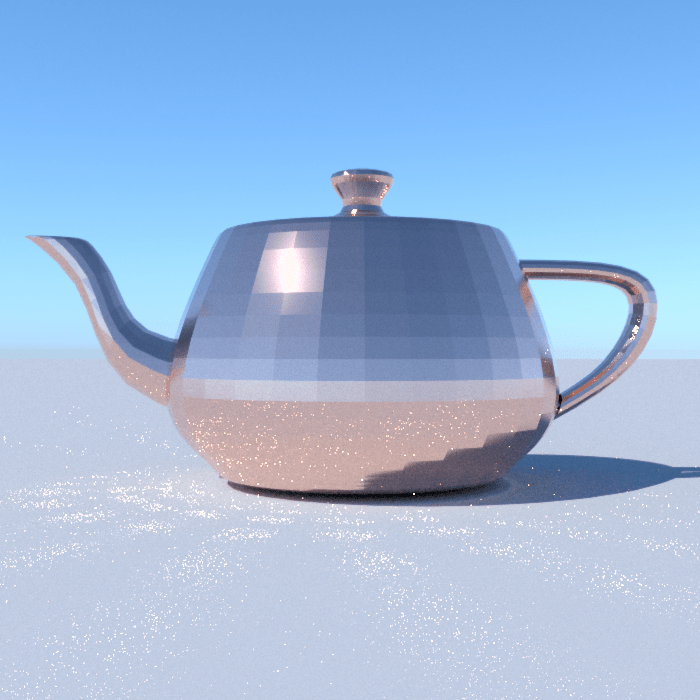
\includegraphics[width=.3\textwidth]{img/4 results/ply/teapotEmbree.png}\label{fig:mesh_teapot}}
	\hfill
	\subfloat[Bunny - 69,451 faces]{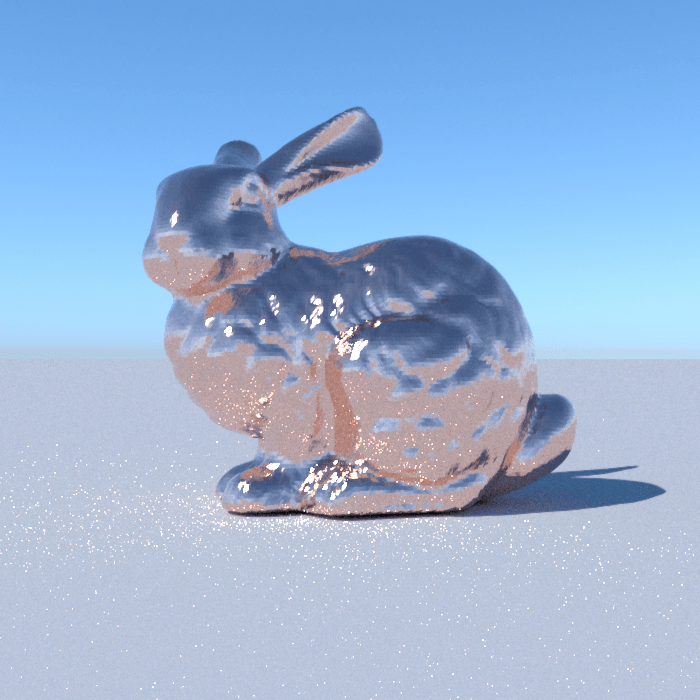
\includegraphics[width=.3\textwidth]{img/4 results/ply/bunnyEmbree.png}\label{fig:mesh_bunny}}
	\hfill
	\subfloat[Michelangelo - 366,011 faces ]{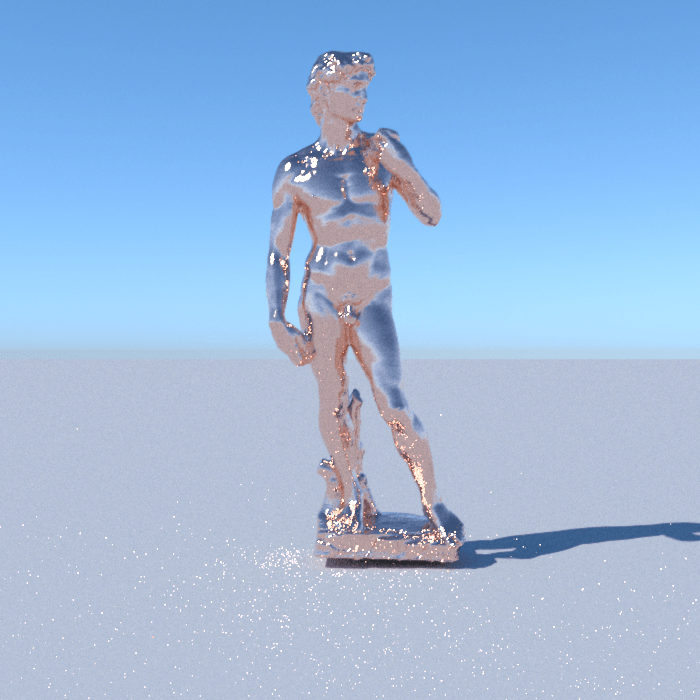
\includegraphics[width=.3\textwidth]{img/4 results/ply/michelangeloEmbree.png}\label{fig:mesh_mike}}
	\\
	\subfloat[Happy Buddha - 1,087,716 faces]{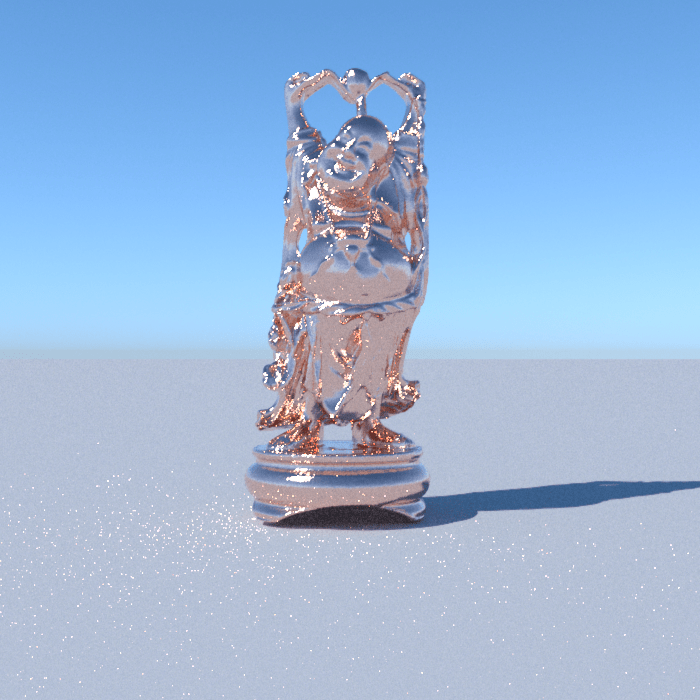
\includegraphics[width=.3\textwidth]{img/4 results/ply/bhuddaEmbree.png}\label{fig:mesh_buddha}}
	\hfill
	\subfloat[Dragon - 7,219,045 faces]{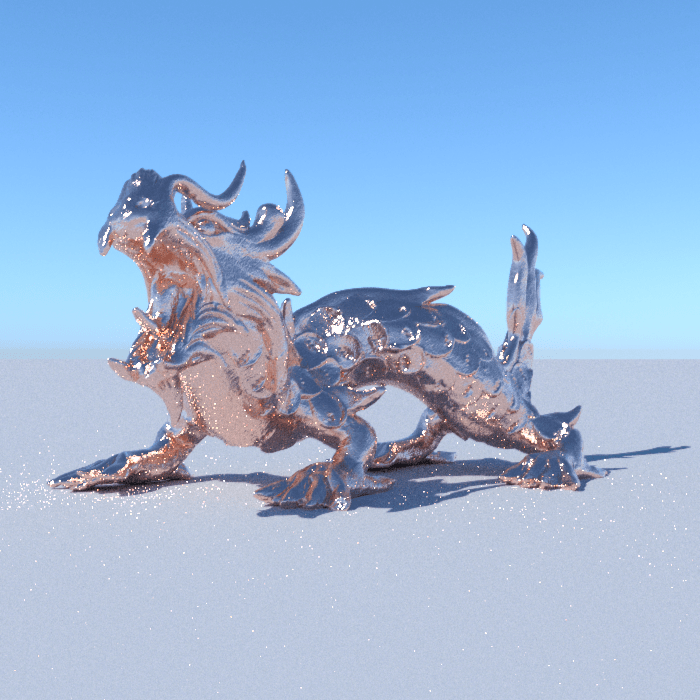
\includegraphics[width=.3\textwidth]{img/4 results/ply/dragonEmbree.png}\label{fig:mesh_dragon}}
	\hfill
	\subfloat[Lucy - 28,055,742 faces ]{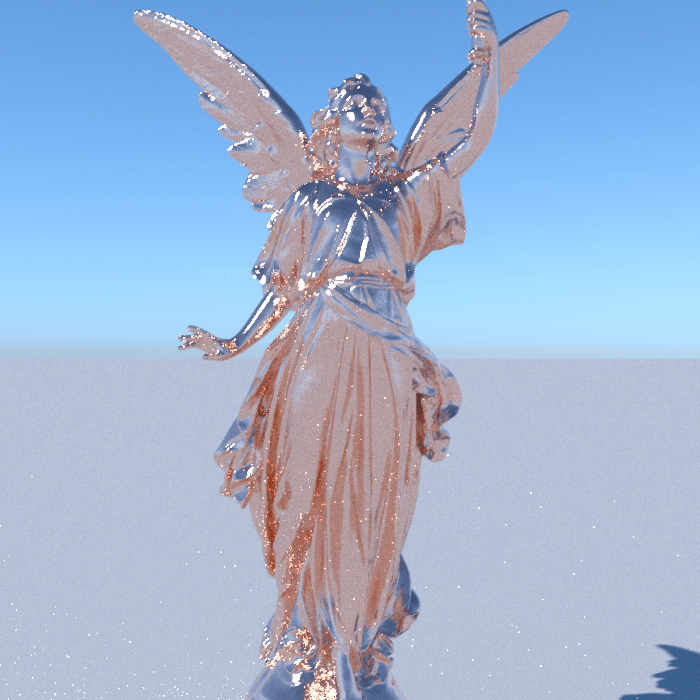
\includegraphics[width=.3\textwidth]{img/4 results/ply/lucyEmbree.png}\label{fig:mesh_lucy}}
	
	\caption{Scenes for triangle meshes}
	\label{fig:mesh_scenes}
\end{figure}

\begin{table}
	\centering
	{\footnotesize\sf
		\begin{tabular}{lrrrr}
			\toprule
			Scene & \Verb!#!Triangles & Native ART & Embree & Speedup \\ 
			\midrule
			Figure \ref{fig:mesh_teapot} & 4,032 & 728.12 sec & 608.29 sec & 16.46 \% \\
			Figure \ref{fig:mesh_bunny} & 69,451 & 379.02 sec & 305.00 sec & 19.53 \% \\
			Figure \ref{fig:mesh_mike} & 366,011 & 302.52 sec & 254.03 sec & 16.03 \%  \\
			\addlinespace % a nice non-intrusive separator of data groups (or final table sums)
			Figure \ref{fig:mesh_buddha} & 1,087,716 & 351.92 sec & 276.00 sec & 21.57 \% \\
			Figure \ref{fig:mesh_dragon} & 7,219,045 & (no data) & 304.29 sec & (no data)  \\
			Figure \ref{fig:mesh_lucy} & 28,055,742 & (no data) & 327.59 sec & (no data)  \\
			\bottomrule
	\end{tabular}}
	\caption{An example table. Table caption should clearly explain how to interpret the data in the table. Use some visual guide, such as boldface or color coding, to highlight the most important results (e.g., comparison winners).}
	\label{tab:mesh}
\end{table}





\begin{figure}
	\centering
	\subfloat[Teapot - 4,032 faces]{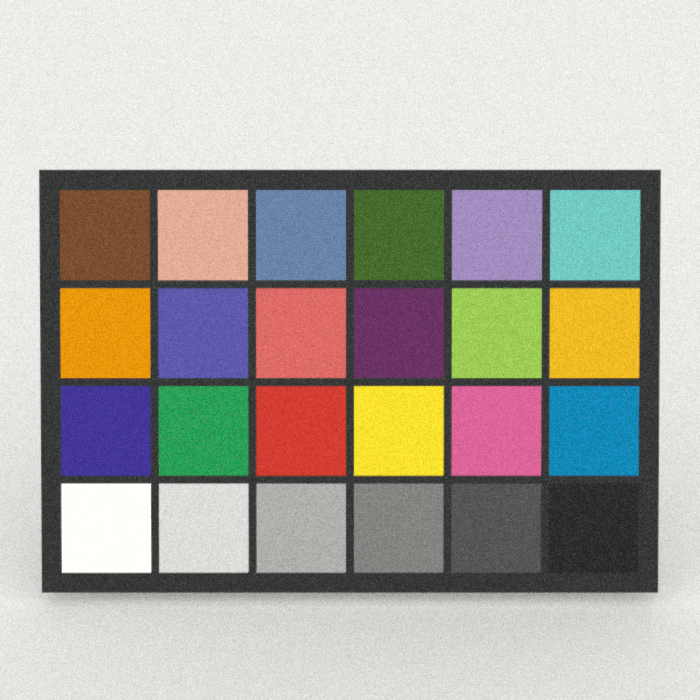
\includegraphics[width=.3\textwidth]{img/4 results/normal/chartEmbree.png}\label{fig:chart}}
	\hfill
	\subfloat[Bunny - 69,451 faces]{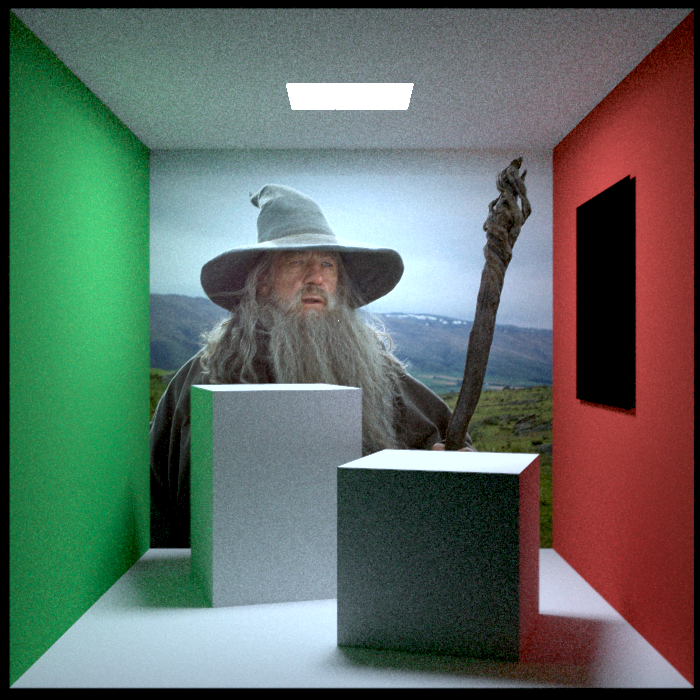
\includegraphics[width=.3\textwidth]{img/4 results/normal/imagemapEmbree.png}\label{fig:gandalf}}
	\hfill
	\subfloat[Michelangelo - 366,011 faces ]{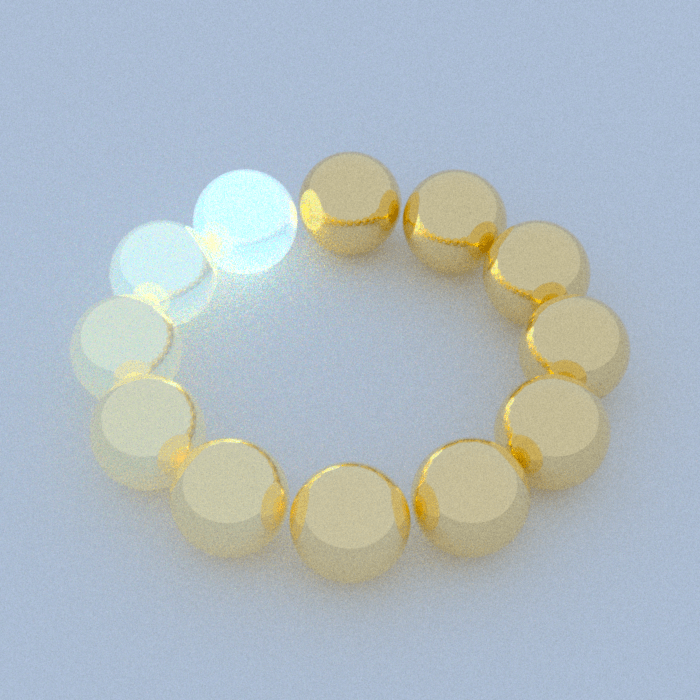
\includegraphics[width=.3\textwidth]{img/4 results/normal/glowEmbree.png}\label{fig:glow}}
	\\
	\subfloat[Happy Buddha - 1,087,716 faces]{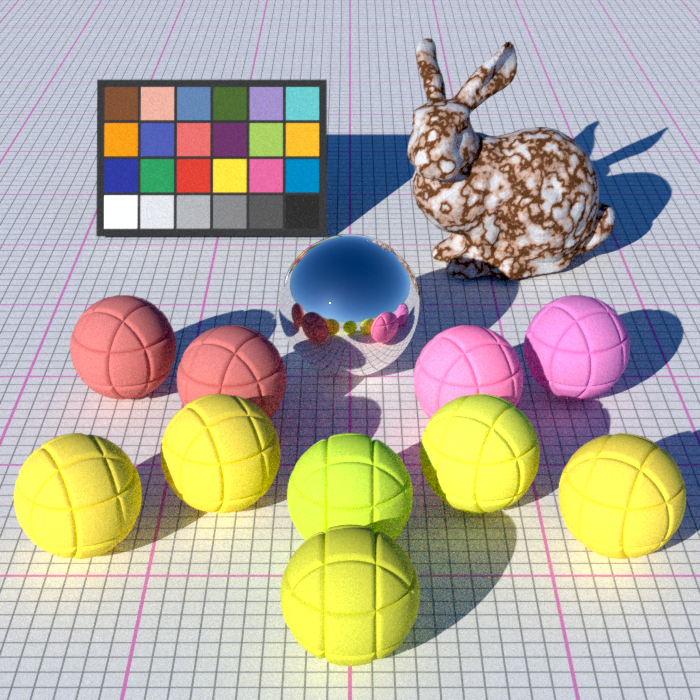
\includegraphics[width=.7\textwidth]{img/4 results/normal/skydomeNormal.png}\label{fig:skydome}}

	
	\caption{Scenes for triangle meshes}
	\label{fig:scenes}
\end{figure}


\begin{table}
	\centering
	{\footnotesize\sf
		\begin{tabular}{lrrrr}
			\toprule
			Scene & \Verb!#!Geometry & Native ART & Embree & Speedup \\ 
			\midrule
			Figure \ref{fig:chart} & 26 & 196.34 sec & 213.15 sec & \textcolor{red}{-8.56 \%} \\
			Figure \ref{fig:gandalf} & 20 & 485.60 sec & 284.27 sec & 41.46 \% \\
			Figure \ref{fig:glow} & 13 & 401.27 sec & 225.29 sec & 43.86 \%  \\
			Figure \ref{fig:skydome} & 38 & - & - & - \\
			\bottomrule
	\end{tabular}}
	\caption{An example table. Table caption should clearly explain how to interpret the data in the table. Use some visual guide, such as boldface or color coding, to highlight the most important results (e.g., comparison winners).}
	\label{tab:scenes}
\end{table}


Rendering triangles and quads, meh.

Not working with Triangle meshes.

